\documentclass[letterpaper,11pt]{article}

\usepackage{amsmath,amssymb,amsthm}
\usepackage[margin=2.0cm]{geometry}
\usepackage{tikz}

\newtheorem{proposition}{Proposition}

\author{Jacob Thomas Errington}
\title{Assignment \#4\\Algorithm Design -- COMP 360}
\date{24 November 2015}

\begin{document}

\maketitle

\begin{enumerate}
    \item
        We know that SAT is in PSPACE. Thus, finding one satisfactory truth
        assignment is in PSPACE. We can then increase a counter and continue
        where we left off. Thus, the only added space comes from the counter.

        The counter can reach a maximum value of $2^n$. Since it takes $\log m$
        bits to write a number $m$ in binary, $n$ bits are required to store
        the maximum value of the counter. Hence, adding this counter to what is
        otherwise a SAT solver requires only a linear amount of space in the
        number of variables, so this new algorithm is also in PSPACE.

    \item
        The optimal solution to this problem can be found by finding the points
        $P$ and $Q$ such that the distance between $P$ and $Q$ is the maximal
        pairwise distance between any two points, placing the center of the
        circle between these two points, and taking the radius to be half the
        distance.

        The proposed algorithm's worst-case performance occurs precisely when
        the first point chosen is either $P$ or $Q$ (since the point furthest
        away from $P$ is $Q$ and they have maximal distance by construction).
        In that case, the radius of the proposed algorithm will be exactly
        twice the optimal radius.

    \item
        We will assume without loss of generality that $\forall i. w_i \leq m$.
        Suboptimal behaviour of the greedy algorithm occurs when it gets to the
        first $i$ for which $w_i + C_i > m$ where $C_i$ is the partial sum
        accumulated before reaching $w_i$. Of course, $w_i \leq C_i$. In the
        worst case, $w_i$ is large, so in particular in the worst case
        $w_i = C_i$. Hence, $2w_i > m$, which implies that $w_i > \frac{m}{2}$.
        Since the optimal value is at most $m$,
        $C_i = w_i > \frac{m}{2} = \frac{\mathrm{opt}}{2}$. Hence, the algorithm
        is a $\frac{1}{2}$-factor approximation.

    \item
        \begin{enumerate}
            \item
                Let the number of clauses in total be $m$, and the number of
                clauses satisfied by some assignment $s$ be $\#_s$. In order
                for a clause to not be satisfied by $\sigma_T$, it must
                consist entirely of negations of variables, for if it contained
                at least one plain variable, then the clause would be
                satisfied. Those clauses not satisfied by the assignment
                $\sigma_T$ would thus be satisfied by $\sigma_F$. Hence,
                $\#_{\sigma_T} = m - \#_{\sigma_F}$. Thus, one of
                $\#_{\sigma_T}$ or $\#_{\sigma_F}$ must be at least half.

            \item
                $x_1 \land \bar x_2$
        \end{enumerate}

    \item Figure \ref{fig:independent-set} shows an example of a graph in which
        the worst-case performance of the greedy algorithm can arise. Indeed,
        for $l < \frac{3w - 1}{4}$, the greedy algorithm is suboptimal. It
        performs more poorly for smaller values of $l$ and most poorly when
        $l = 1$, in which case the score of the independent set that it chooses
        can be no more than four times worse than the score of the optimal
        independent set.

        In a more general setting, suppose that the score of the independent
        set chosen by the greedy algorithm is more than four times worse than
        the optimal score. Then, there would need to be some subgraph of size
        $3 \times 3$ in which it locally performed more than four times worse,
        which is not possible. Hence, the greedy algorithm produces an
        independent set whose score is at least $\frac{1}{4}$ times the maximal
        score over all independent sets in the grid graph $G$.

        \begin{figure}[ht]
            \centering
            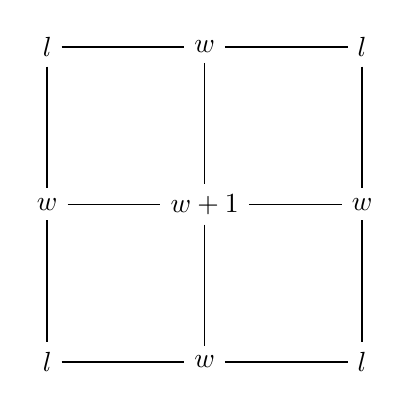
\begin{tikzpicture}[
                    -,
                    auto,
                    node distance=2.0cm,
                    semithick
                ]
                \node (11) {$l$} ;
                \node (12) [right of=11] {$w$} ;
                \node (13) [right of=12] {$l$} ;
                \node (21) [below of=11] {$w$} ;
                \node (22) [below of=12] {$w + 1$} ;
                \node (23) [below of=13] {$w$} ;
                \node (31) [below of=21] {$l$} ;
                \node (32) [below of=22] {$w$} ;
                \node (33) [below of=23] {$l$} ;

                \path
                (11) edge node {} (12)
                (11) edge node {} (21)
                (12) edge node {} (13)
                (12) edge node {} (22)
                (13) edge node {} (23)
                (21) edge node {} (22)
                (21) edge node {} (31)
                (22) edge node {} (23)
                (22) edge node {} (32)
                (23) edge node {} (33)
                (31) edge node {} (32)
                (32) edge node {} (33)
                ;
            \end{tikzpicture}

            \caption{
                The simplest graph exhibiting the worst-case performance of the
                greedy algorithm. In this example, $l < w$. The independent set
                chosen by the greedy algorithm would have score $w + 4l + 1$.
                The other interesting choice of independent set would have
                score $4w$.
            }
            \label{fig:independent-set}
        \end{figure}

    \item
        \begin{enumerate}
            \item
                Vertices are assigned the value $1$ when they are removed, and
                assigned $0$ when they are kept. Since the objective function
                represents the number of removed vertices and this is a
                minimization problem, the number of vertices to remove will be
                minimized.

                Each variable is constrained to be in the set $\{0, 1\}$,
                ensuring that illegal values are not assigned. Then, for each
                cycle in $\mathcal{C}_4$, at least one variable must have the
                value $1$ assigned, representing its removal, which guarantees
                that each cycle is broken.

            \item
                Suppose that a variable $x_1 \in C$ for some
                $C \in \mathcal{C}_4$ were assigned the value $w > 1$. Reducing
                its assigned value to $1$ would not violate any constraints;
                any sum including $x_1$ as a term would still come out to at
                least $1$. Furthermore, reducing the value to $1$ would improve
                the objective function, since this is a minimization problem.
                Hence, although the feasible region of the linear program
                includes solutions with values for $x_i > 1$, those solutions
                are never optimal, so the solver will never emit such a
                solution as output.

            \item
                First, we notice that an extremely naive $4$-factor
                approximation would simply be to remove all $v \in C$ for all
                $C \in \mathcal{C}_4$. Indeed, each $C \in \mathcal{C}_4$ is
                such that $|C| = 4$, so removing all of those vertices removes
                at most $4$ times the necessary number of vertices per cycle,
                and hence at most $4$ times the total necessary number of
                vertices.

                Our $4$-factor approximation based on the output of the linear
                program is simply to take the ceiling of all the variables. The
                worst this can do is remove all vertices, which as we have
                shown above is already a $4$-factor approximation.

            \item
                First, notice that for all $C \in \mathcal{C}_4$, two vertices
                lie in $L$ and the other two lie in $R$.
                Now, suppose that $\hat x$ is not a feasible solution to the
                integer program. The rounding procedure ensures that all
                variables have either the value $0$ or the value $1$, so that
                constraint is certainly satisfied. Hence, there must be some
                $C \in \mathcal{C}_4$ such that $\sum_{u \in C} \hat x_u < 1$.
                In order for that to be the case, the two variables
                corresponding to the two vertices in $L$ must have been exactly
                zero, and the two variables corresponding to the two vertices
                in $R$ must have been strictly less than half. However, that is
                a contradtiction of the constraint $\sum_{u \in C} x_u \geq 1$
                of the linear program. Thus, all optimal solutions to the
                linear program are feasible solutions to the integer program.

            \item
                First, notice that for all $C \in \mathcal{C}_4$, since
                $|C| = 4$, we have the following.
                $$
                |\{u \in C | \hat x_u = 1\}| \leq 4
                $$

                Also, the exclusive-or formulation of the statement to show is
                logically equivalent to an if-and-only-if statement with one
                side negated, so that is what we will prove.

                \begin{proposition}
                    For every $C \in \mathcal{C}_4$,
                    $$
                    |\{u \in C | \hat x_u = 1\}| \leq 3 \iff y_C^* > 0
                    $$
                \end{proposition}

                \begin{proof}
                    We will first show that the right-hand side implies the
                    left-hand side by proving the contrapositive, i.e. that
                    $\{u \in C | \hat x_u = 1\}| > 3 \implies y_C^* = 0$.

                    Suppose that for some $C$, we have
                    $|\{u \in C | \hat x_u = 1\}| > 3$.
                    Then for each vertex in $C$, its corresponding variable was
                    rouded up. That requires that the two variables
                    corresponding to vertices in $R$ had values at least
                    $\frac{1}{2}$, and the two variables corresponding to
                    vertices in $L$ had values greater than $0$. The sum of
                    those four variables is \emph{strictly} greater than $1$,
                    so there is slack in that constraint. By the complementary
                    slackness theorem, the corresponding dual variable
                    $y_C^* = 0$.

                    Now we will show that the left-hand side implies the
                    right-hand side, i.e. that
                    \begin{equation*}
                        y_C^* > 0 \implies |\{u \in C | \hat x_u = 1\}| \leq 3
                    \end{equation*}

                    By the completementary slackness theorem, we can instead
                    prove
                    \begin{equation*}
                        \sum_{u \in C} x_u = 1
                        \implies
                        |\{u \in C | \hat x_u = 1\}| \leq 3
                    \end{equation*}

                    We know $|C| = 4$, so let $v_1, v_2, v_3, v_4 \in C$. Hence,
                    $x_1 + x_2 + x_3 + x_4 = 1$. Suppose futhermore that
                    $x_1, x_2 \in C_R$ and $x_3, x_4 \in C_L$, where $C_R$ and
                    $C_L$ are the subgraphs of $C$ whose vertices lie in $R$
                    and in $L$, respectively.

                    Suppose that all four variables were rounded. In order for
                    that to occur,
                    \begin{align*}
                        x_1 &> \frac{1}{2} \\
                        x_2 &> \frac{1}{2} \\
                        x_3 &> 0 \\
                        x_4 &> 0
                    \end{align*}
                    but this sum is greater that $1$, which contradicts the
                    premise of the implication. Hence, no more than $3$ of the
                    variables can be rounded in order for there to be no slack.
                \end{proof}

            \item
                Let $m = |\mathcal{C}_4|$ and $0 \leq n \leq m$ be the number
                of contraints having slack, i.e. in which all variables have
                been rounded up. Then $m - n$ is the number of nonzero dual
                variables. Each dual variable is at most $1$, so by strong
                duality, we have that
                $x^* = y^* \leq m - n \implies x^* + n \leq m$

        \end{enumerate}
\end{enumerate}
\end{document}
